\chapter{Background and Literature Review}
\label{ch:background}
\glsresetall
{
Chapter starting text here.}

\section{First Section Title Here}
\label{sec:sectionRefNameHere}

\begin{figure}[tb!] % "tb!" puts it at top, if possible, then at bottom. the "!" tries harder to put it where you place it. Make every effort to have Figures at/after the first reference and within 1 page distance of the first reference, if possible.
	\centering
	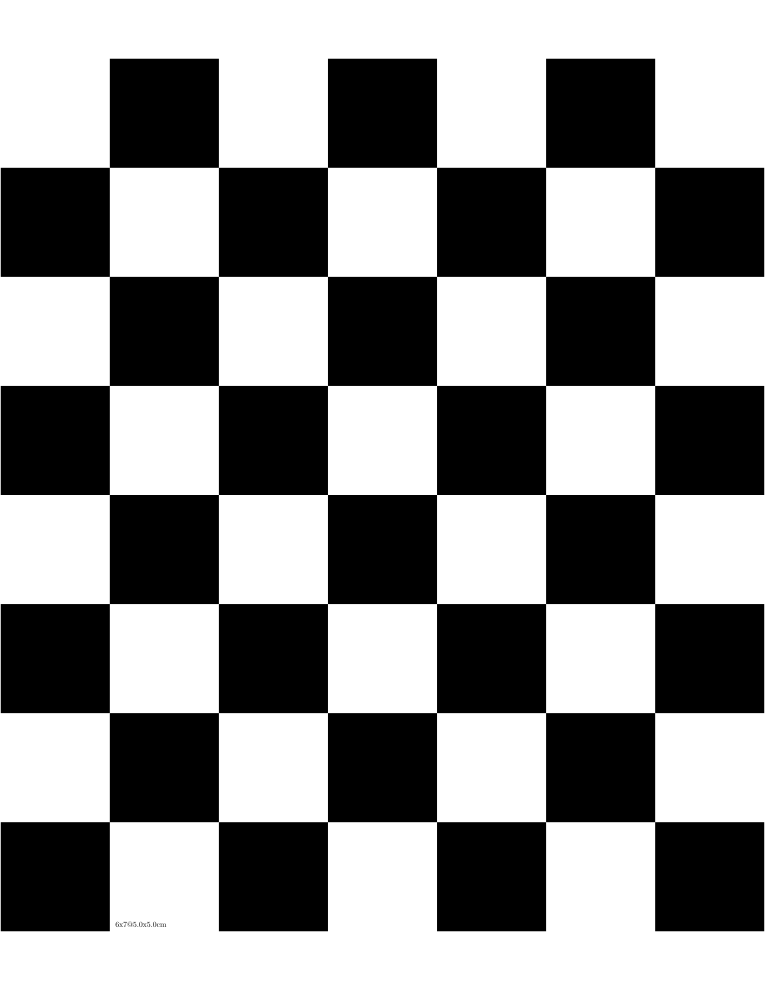
\includegraphics[width = 0.75\columnwidth]{Figures/checkerboard7x6x50x50cm.png}
	\caption[TOC Figure Name]{Title shown in text here: short paragraph description of picture here}
	\label{fig:examplePicture}
\end{figure}

Text description here, can reference other Chapters or Sections, like \Cref{ch:introduction} or \Cref{fig:examplePicture}.

\subsection[Optional TOC Subsection Title Here]{Subsection Title Here}
\label{sec:subsectionRefNameHere}
\phantomsection

Take about an equation with text without space, like
\begin{equation}
\label{eq:eqRefNameHere}
%\lambda 
\frac{1}{z}
\begin{bmatrix}
u \\
v \\
1 \\
\end{bmatrix}=
K \begin{bmatrix}
x \\
y \\
z \\
\end{bmatrix}=
\begin{bmatrix}
f_x & 0 & c_x \\
0 & f_y & c_y \\
0 & 0 & 1 \\
\end{bmatrix}
\begin{bmatrix}
x \\
y \\
z \\
\end{bmatrix}
\end{equation}
where $\lambda$ can be referenced. Don't put lines before or after equations, unless the equation is the end of a paragraph's discussion. 

You can also include an algorithm, like \Cref{alg:algorithmRefName}. 

\begin{algorithm}[tb!]
	\caption{Algorithm Title Here}
	\label{alg:algorithmRefName}
	\begin{algorithmic}[1] % The number tells where the line numbering should start
		\Function{foo}{$a,b,c$}
		\State $\mathbf{R}^{C_0}_W,\mathbf{p}^W_{C_0} \gets \textsc{getPose}(e_0.t)$	\Comment{Target pose}	
		\For{$k\gets 1,N$} \Comment{Loop over events}
		\State $\begin{bmatrix}x_H \\ y_H \end{bmatrix}  \gets \textsc{undistPos}(e_x,e_y)$ \Comment Pixel location to position
		\label{alg:line:lineRefName} % to use to reference specific lines in Algorithm
		\EndFor
		\State \textbf{return} $image$\Comment{Output}
		\EndFunction
	\end{algorithmic}
\end{algorithm}
